\documentclass[border=12pt]{standalone}
\usepackage{tikz}
\usetikzlibrary{shapes.geometric, arrows.meta, positioning, calc, fit, backgrounds}
\usepackage{fontspec}
\usepackage{amsmath,amssymb}
\setmainfont{DejaVu Sans}

\begin{document}
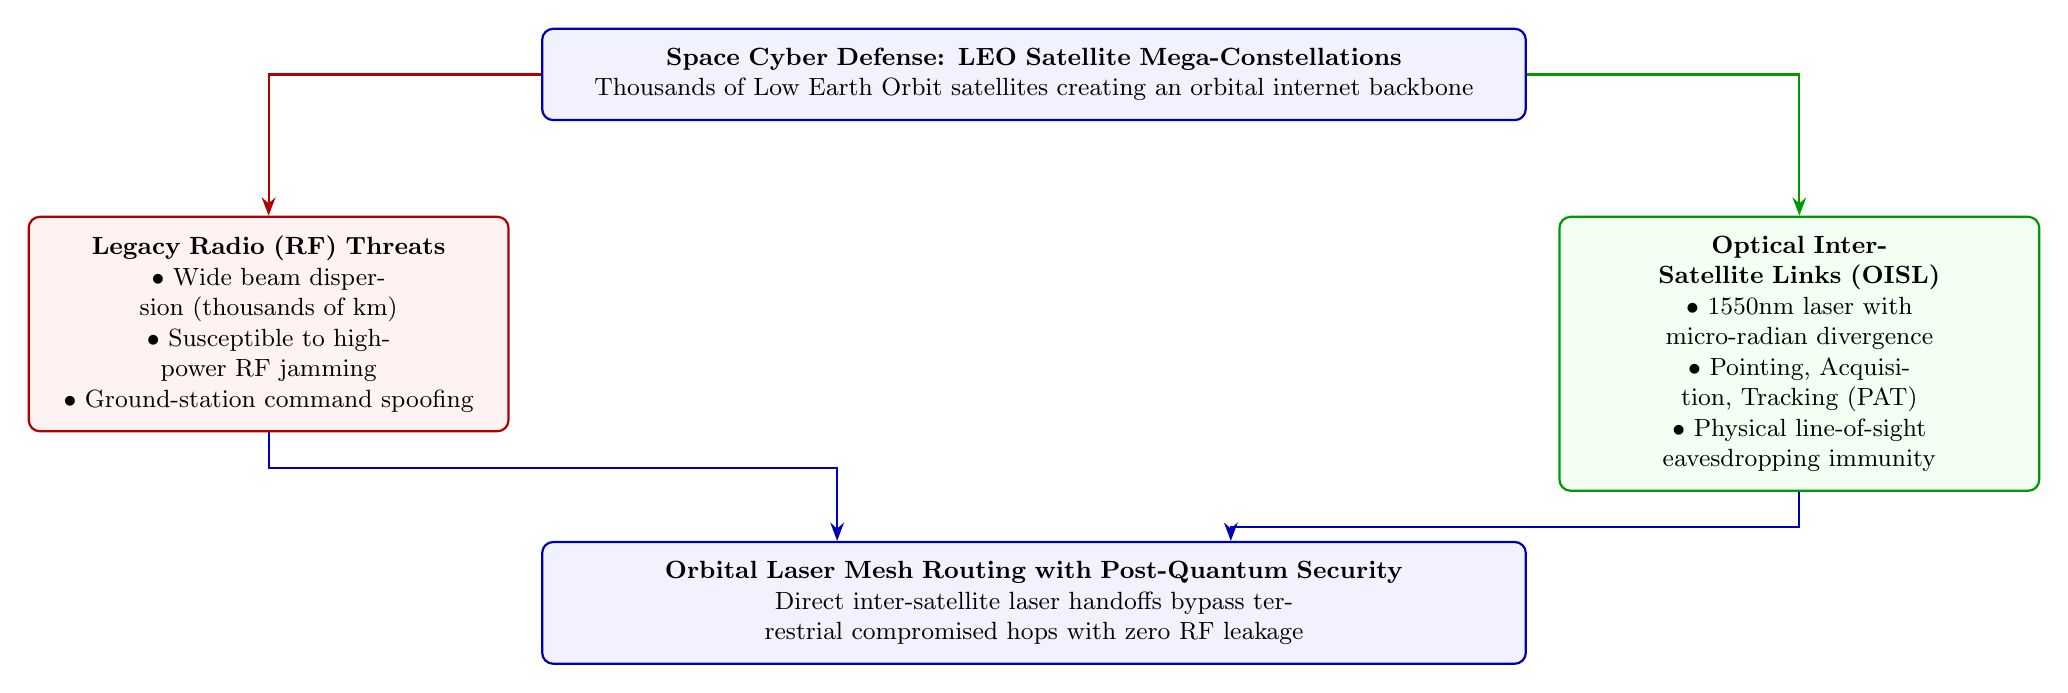
\begin{tikzpicture}[
    font=\small,
    >=Stealth,
    node distance=1.2cm,
    block/.style={rectangle, draw=blue!70!black, fill=blue!5, rounded corners=4pt, thick, align=center, inner sep=7pt},
    alertblock/.style={rectangle, draw=red!70!black, fill=red!5, rounded corners=4pt, thick, align=center, inner sep=7pt},
    greenblock/.style={rectangle, draw=green!60!black, fill=green!5, rounded corners=4pt, thick, align=center, inner sep=7pt},
    amberblock/.style={rectangle, draw=orange!80!black, fill=orange!5, rounded corners=4pt, thick, align=center, inner sep=7pt}
]

\node[block, text width=12cm] (top) {\textbf{Space Cyber Defense: LEO Satellite Mega-Constellations}\\Thousands of Low Earth Orbit satellites creating an orbital internet backbone};

\node[alertblock, below left=1.2cm and 0.4cm of top, text width=5.6cm] (rf) {\textbf{Legacy Radio (RF) Threats}\\$\bullet$ Wide beam dispersion (thousands of km)\\$\bullet$ Susceptible to high-power RF jamming\\$\bullet$ Ground-station command spoofing};

\node[greenblock, below right=1.2cm and 0.4cm of top, text width=5.6cm] (oisl) {\textbf{Optical Inter-Satellite Links (OISL)}\\$\bullet$ 1550nm laser with micro-radian divergence\\$\bullet$ Pointing, Acquisition, Tracking (PAT)\\$\bullet$ Physical line-of-sight eavesdropping immunity};

\node[block, below=1.0cm of $(rf.south)!0.5!(oisl.south)$, text width=12cm] (bottom) {\textbf{Orbital Laser Mesh Routing with Post-Quantum Security}\\Direct inter-satellite laser handoffs bypass terrestrial compromised hops with zero RF leakage};

\draw[->, thick, red!70!black] (top) -| (rf);
\draw[->, thick, green!60!black] (top) -| (oisl);
\draw[->, thick, blue!70!black] (rf.south) -- ++(0,-0.45) -| ([xshift=-2.5cm]bottom.north);
\draw[->, thick, blue!70!black] (oisl.south) -- ++(0,-0.45) -| ([xshift=2.5cm]bottom.north);

\end{tikzpicture}
\end{document}
